\documentclass{article}
\usepackage{natbib}
\usepackage[utf8]{inputenc}
\usepackage{hyperref}
\usepackage{graphicx}

\usepackage{amsmath}
\usepackage{amssymb}

\def \N {\mathbb{N}}
\def \Nbr {\mathcal{N}}
\def \Q {\mathbb{Q}}
\def \F {\mathbb{F}}
\def \then {\implies &}
\def \oif {\Longleftrightarrow &\,}
\def \given {\text{Given }&}
\def \assume {\text{Assume }&}
\def \thfr {\therefore &\enskip}
\def \bij {\leftrightarrow}
\def \inj {\rightarrowtail}
\def \sur {\twoheadedrightarrow}
\def \Z {\mathbb{Z}}
\def \R {\mathbb{R}}
\def \C {\mathbb{C}}
\def \D {\mathbb{D}}
\def \H {\mathbb{H}}
\def \iff {\Longleftrightarrow}
\def \kron {\boldsymbol\delta}
\def \id {\text{id}}

\def\Tx{\textbf{x}}
\def\Ty{\textbf{y}}
\def\quotient{\mathclose{}/\mathopen{}}
\def\Tf{\textbf{f}}
\def\Th{\textbf{h}}
\def\Tg{\textbf{g}}
\def\sumn{\sum_{n=0}^\infty}
\def\limn{\lim_{n\rightarrow\infty}}
\def\prodn{\prod_{n=0}^\infty}
\DeclareMathOperator\adj{adj}

\newcommand{\stc}[1]{\widetilde{#1}}   
\newcommand{\pa}[1]{ \left({#1}\right) }
\newcommand{\set}[2]{ \left\{ #1 \,\middle|\, #2 \right\} }
\newcommand{\shift}[1]{&\quad & \text{#1}\\}
\newcommand{\lem}[1]{\text{\textbf{L.\ref{#1}}}}
\newcommand{\card}[1]{\left\vert{#1}\right\vert}
\newcommand{\Ps}[1]{\mathcal{P}\left({ #1 }\right)}
\newcommand{\colv}[1]{\begin{pmatrix} #1 \end{pmatrix}}
\newcommand{\mat}[1]{\begin{pmatrix} #1 \end{pmatrix}}
\newcommand{\detmat}[1]{\begin{vmatrix} #1 \end{vmatrix}}
\newcommand{\spanb}[1]{\text{span}\{ #1 \}}
\newcommand{\abs}[1]{\left|#1\right|}
\newcommand{\Inner}[1]{\langle #1 \rangle}
\newcommand{\Innercpy}[1]{\langle #1, #1 \rangle}
\newcommand{\conj}[1]{{\overline{#1}}}

\DeclareMathOperator{\Tr}{tr}
\DeclareMathOperator{\Dim}{dim}
\DeclareMathOperator{\Rank}{rank}
\DeclareMathOperator{\Ker}{ker}
\DeclareMathOperator{\Diam}{diam}
\DeclareMathOperator{\Diag}{diag}
\DeclareMathOperator{\Int}{int}
\DeclareMathOperator{\Clo}{clo}
\DeclareMathOperator{\sgn}{sgn}
\DeclareMathOperator{\MyRe}{Re}
\DeclareMathOperator{\MyIm}{Im}
\DeclareMathOperator{\res}{res}

%\usepackage{enumerate}
%\renewcommand{\theenumi}{\alph{enumi}}
%\renewcommand{\theenumii}{\roman{enumii}}

\title{COS513 Finance}
\author{ }
\date{}

\begin{document}

\maketitle

Financial data prediction is appealing both for its challenging nature and for its practical applications. Because market dynamics are complex and random, accurate price prediction is difficult. There are two types of market prediction techniques: fundamental analysis, which relies on an asset's data for forecasting, and technical analysis, which relies on historical trends to exploit market timing \cite{schumaker2009textual}. This paper examines the use of news data to augment technical analysis for prediction of commodity prices. We assume there is a set of news basis vectors that is stable over time which can be used for this purpose. %TODO: keep last sentence?

We focus on a comprehensive set of non-economic news data unrelated to financial markets, interest rates, stock prices, and the like. In particular, we will analyze whether a summary of a day's news topics is predictive of commodity prices the next day. To avoid losing information about the significance of singular events, we will rely on the sentiment analysis already applied to our dataset to calculate how each news event should be weighted in a daily news summary.

\subsection{Commodity Prediction}
We choose to predict commodities prices because while various studies have analyzed the effect of news on stock prices \cite{mcqueen1993stock} and foreign exchange rates \cite{kamruzzaman2003svm}, relatively little work has looked at applying news data to the prediction of the similar commodities market. The use non-economic news because the influence of economic news has already been examined in the past by many researchers \cite{gidofalvi2001using}\cite{schumaker2009textual}\cite{bollen2011twitter}\cite{hagenau2012automated}. We believe real-time news information has predictive power for commodity prices, because, since commodities, by definition, must be extracted or produced by countries, it is likely that underlying factors of their production rates will be captured by local news, especially reporting on crisis events. Prices are also sensitive to current conditions because the supply and demands that drive them are inelastic, or unaffected by changes in price \cite{chen2008can}. 

\subsection{GDELT Dataset}
We draw news from the Global Database of Events, Language, and Tone \cite{GDELT}, which aggregates news from broadcast, print, and web sources across 100 languages and parses out features to describe each news event. Each news event has 58 features which can be broadly divided into either topical or importance-related data. Topical data might include the two actors involved in an event, the general sentiment of the language used, the location of actors, or broad categorization of the type of event occurring (trade agreement, violent action, etc) in categorical codes (CAMEO codes). Importance-related features deal with the magnitude of the event and are drawn from metrics such as the number of news sources mentioning the event, or the total number of articles written about it. GDELT is available for free and uses a variety of international news sources with daily updates, and contains more than 250 million events from 1979 to present, or roughly 100,000 per day. GDELT's predictive potential for financial markets has been positively assessed by researchers who used GDELT to examine the impacts of the June 2013 Southeast Asian heat wave and the December 2013 Indian riots and the effect they had on the Singapore stock market \cite{phua2014visual}.


\section{Background}

\subsection{Dimensionality Reduction for Categorical Data}

blah blah

tsne \cite{van2008visualizing}.


\section{Related Work}



analysis done on prefix of days to prevent overfitting \cite{leetaru2013gdelt}

(summary info, description of columns)

(description of columns we actually used)

\begin{figure}[ht]
\vskip 0.2in
\begin{center}
\centerline{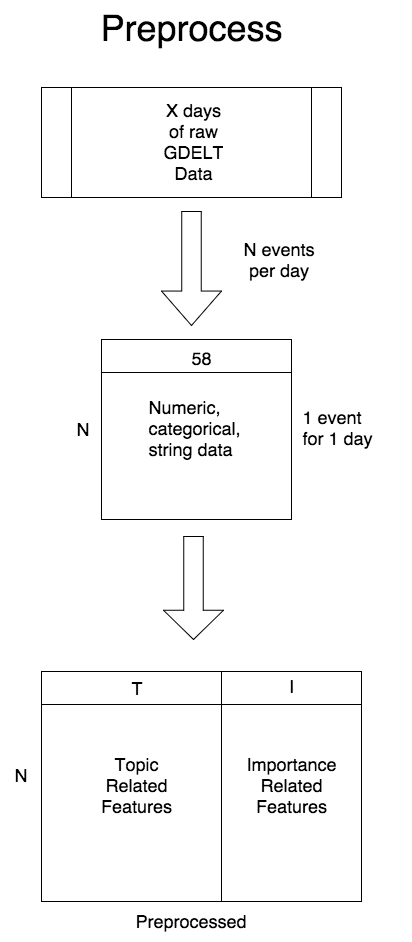
\includegraphics[scale=0.15]{images/preprocess_vertical.png}}
\caption{Preprocess stage}
\end{center}
\vskip -0.2in
\label{fig:preprocess}
\end{figure} 


\begin{figure}[ht]
\vskip 0.2in
\begin{center}
\centerline{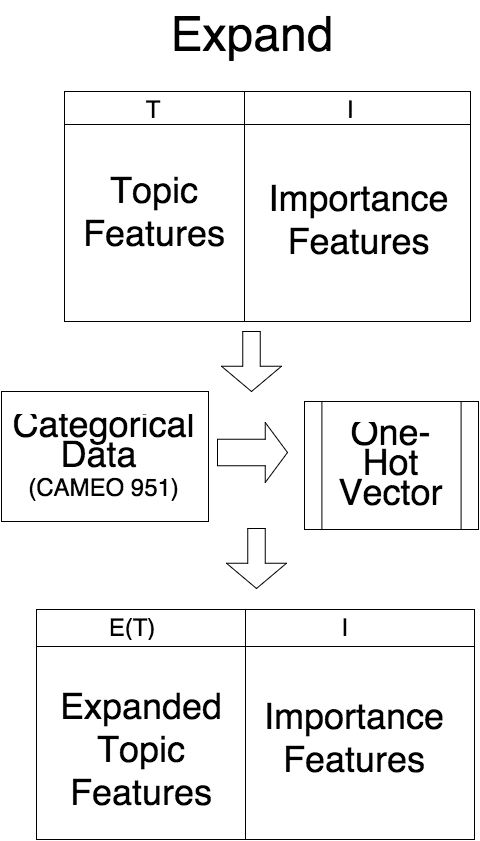
\includegraphics[width=\columnwidth]{images/expand_vertical.png}}
\caption{Expand stage}
\end{center}
\vskip -0.2in
\label{fig:exapand}
\end{figure} 




\begin{figure}[ht]
\vskip 0.2in
\begin{center}
\centerline{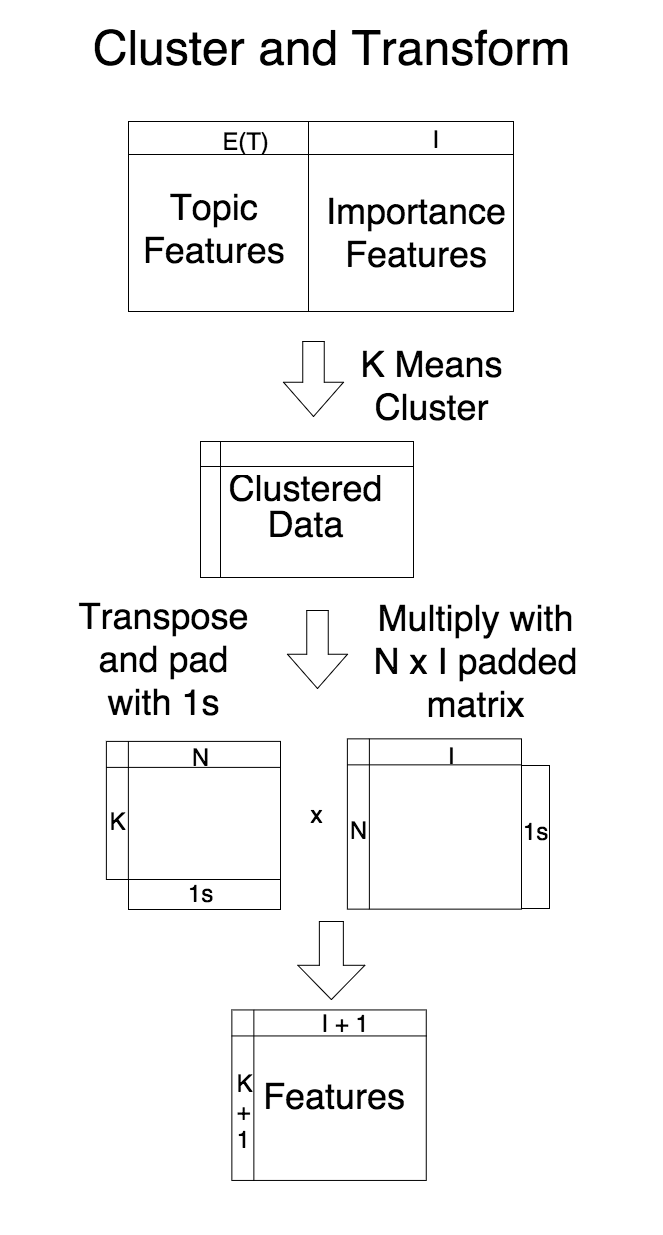
\includegraphics[scale=0.15]{images/cluster_and_transform_vertical.png}}
\caption{Summarization stage}
\end{center}
\vskip -0.2in
\label{fig:summarization}
\end{figure} 
% Other inputs

\pagebreak
\bibliographystyle{plain}
\bibliography{biblio.bib}

\end{document}
